\documentclass[]{article}

\usepackage{amsmath,amssymb}
\usepackage{amsthm}

\usepackage{graphicx,xcolor}

\usepackage{algorithm,algpseudocode,float} 

\renewcommand\thesubsubsection{\Alph{subsubsection})}

\newtheorem{proposition}{Proposition}

%opening
\title{Optimal partition assignment in Garage}
\author{Mendes}

\begin{document}

\maketitle

\section{Introduction}

\subsection{Context}

Garage is an open-source distributed storage service blablabla$\dots$

Every object to be stored in the system falls in a partition given by the last $k$ bits of its hash. There are $P=2^k$ partitions. Every partition will be stored on distinct nodes of the system. The goal of the assignment of partitions to nodes is to ensure (nodes and zone) redundancy and to be as efficient as possible.

\subsection{Formal description of the problem}

We are given a set of nodes $\mathbf{N}$ and a set of zones $\mathbf{Z}$. Every node $n$ has a non-negative storage capacity $c_n\ge 0$ and belongs to a zone $z\in \mathbf{Z}$. We are also given a number of partition $P>0$ (typically $P=256$).

We would like to compute an assignment of nodes to partitions. We will impose some redundancy constraints to this assignment, and under these constraints, we want our system to have the largest storage capacity possible. To link storage capacity to partition assignment, we make the following assumption:
\begin{equation}
	\tag{H1}
	\text{\emph{All partitions have the same size $s$.}}
\end{equation}
This assumption is justified by the dispersion of the hashing function, when the number of partitions is small relative to the number of stored large objects.

Every node $n$ wille store some number $k_n$ of partitions. Hence the partitions stored by $n$ (and hence all partitions by our assumption) have there size bounded by $c_n/k_n$. This remark leads us to define the optimal size that we will want to maximize:

\begin{equation}
	\label{eq:optimal}
	\tag{OPT}
s^* = \min_{n \in N} \frac{c_n}{k_n}.
\end{equation}

When the capacities of the nodes are updated (this includes adding or removing a node), we want to update the assignment as well. However, transferring the data between nodes has a cost and we would like to limit the number of changes in the assignment. We make the following assumption:
\begin{equation}
	\tag{H2}
	\text{\emph{Updates of capacity happens rarely relatively to object storing.}}
\end{equation}
This assumption justifies that when we compute the new assignment, it is worth to optimize the partition size \eqref{eq:optimal} first, and then, among the possible optimal solution, to try to minimize the number of partition transfers.

For now, in the following, we ask the following redundancy constraint:

\textbf{Parametric node and zone redundancy:} Given two integer parameters $1\le \rho_\mathbf{Z} \le \rho_\mathbf{N}$, we ask every partition to be stored on $\rho_\mathbf{N}$ distinct nodes, and these nodes must belong to at least $\rho_\mathbf{Z}$ distinct zones.


\textbf{Mode 3-strict:}  every partition needs to be assignated to three nodes belonging to three different zones.

\textbf{Mode 3:} every partition needs to be assignated to three nodes. We try to spread the three nodes over different zones as much as possible.

\textbf{Warning:} This is a working document written incrementaly. The last version of the algorithm is the \textbf{parametric assignment} described in the next section.


\section{Computation of a parametric assignment}
\textbf{Attention : }We change notations in this section.

Notations : let $P$ be the number of partitions, $N$ the number of nodes, $Z$ the number of zones. Let $\mathbf{P,N,Z}$ be the label sets of, respectively, partitions, nodes and zones.
Let $s^*$ be the largest partition size achievable with the redundancy constraints. Let $(c_n)_{n\in \mathbf{N}}$ be the storage capacity of every node. 

In this section, we propose a third specification of the problem. The user inputs two redundancy parameters $1\le \rho_\mathbf{Z} \le \rho_\mathbf{N}$. We compute an assignment $\alpha = (\alpha_p^1, \ldots, \alpha_p^{\rho_\mathbf{N}})_{p\in \mathbf{P}}$ such that every partition $p$ is associated to $\rho_\mathbf{N}$ distinct nodes $\alpha_p^1, \ldots, \alpha_p^{\rho_\mathbf{N}}$ and these nodes belong to at least $\rho_\mathbf{Z}$ distinct zones.

If the layout contained a previous assignment $\alpha'$, we try to minimize the amount of data to transfer during the layout update by making $\alpha$ as close as possible to $\alpha'$.

In the following subsections, we describe the successive steps of the algorithm we propose to compute $\alpha$.

\subsubsection*{Algorithm}

\begin{algorithmic}[1]
	\Function{Compute Layout}{$\mathbf{N}$, $\mathbf{Z}$, $\mathbf{P}$, $(c_n)_{n\in \mathbf{N}}$, $\rho_\mathbf{N}$, $\rho_\mathbf{Z}$, $\alpha'$}
	\State $s^* \leftarrow$ \Call{Compute Partition Size}{$\mathbf{N}$, $\mathbf{Z}$, $\mathbf{P}$, $(c_n)_{n\in \mathbf{N}}$, $\rho_\mathbf{N}$, $\rho_\mathbf{Z}$}
	\State $G \leftarrow G(s^*)$
	\State $f \leftarrow$ 	\Call{Compute Candidate Assignment}{$G$, $\alpha'$}
	\State $f^* \leftarrow$ 	\Call{Minimize transfer load}{$G$, $f$, $\alpha'$}
	\State Build $\alpha^*$ from $f^*$
	\State \Return $\alpha^*$
	\EndFunction
\end{algorithmic}

\subsubsection*{Complexity}
As we will see in the next sections, the worst case complexity of this algorithm is $O(P^2 N^2)$. The minimization of transfer load is the most expensive step, and it can run with a timeout since it is only an optimization step. Without this step (or with a smart timeout), the worst cas complexity can be $O((PN)^{3/2}\log C)$ where $C$ is the total storage capacity of the cluster. 

\subsection{Determination of the partition size $s^*$}

Again, we will represent an assignment $\alpha$ as a flow in a specific graph $G$. We will not compute the optimal partition size $s^*$ a priori, but we will determine it by dichotomy, as the largest size $s$ such that the maximal flow achievable on $G=G(s)$ has value $\rho_\mathbf{N}P$. We will assume that the capacities are given in a small enough unit (say, Megabytes), and we will determine $s^*$ at the precision of the given unit.

Given some candidate size value $s$, we describe the oriented weighted graph $G=(V,E)$ with vertex set $V$ arc set $E$.

The set of vertices $V$ contains the source $\mathbf{s}$, the sink $\mathbf{t}$, vertices 
$\mathbf{p^+, p^-}$ for every partition $p$, vertices $\mathbf{x}_{p,z}$ for every partition $p$ and zone $z$, and vertices $\mathbf{n}$ for every node $n$. 

The set of arcs $E$ contains:
\begin{itemize}
	\item ($\mathbf{s}$,$\mathbf{p}^+$, $\rho_\mathbf{Z}$) for every partition $p$;
	\item ($\mathbf{s}$,$\mathbf{p}^-$, $\rho_\mathbf{N}-\rho_\mathbf{Z}$) for every partition $p$;
	\item ($\mathbf{p}^+$,$\mathbf{x}_{p,z}$, 1) for every partition $p$ and zone $z$;
	\item ($\mathbf{p}^-$,$\mathbf{x}_{p,z}$, $\rho_\mathbf{N}-\rho_\mathbf{Z}$) for every partition $p$ and zone $z$;
	\item ($\mathbf{x}_{p,z}$,$\mathbf{n}$, 1) for every partition $p$, zone $z$ and node $n\in z$;
	\item ($\mathbf{n}$, $\mathbf{t}$, $\lfloor c_n/s \rfloor$) for every node $n$.
\end{itemize}

In the following complexity calculations, we will use the number of vertices and edges of $G$. Remark from now that $\# V = O(PZ)$ and $\# E = O(PN)$.

\begin{proposition}
	An assignment $\alpha$ is realizable with partition size $s$ and the redundancy constraints $(\rho_\mathbf{N},\rho_\mathbf{Z})$ if and only if there exists a maximal flow function $f$ in $G$ with total flow $\rho_\mathbf{N}P$, such that the arcs ($\mathbf{x}_{p,z}$,$\mathbf{n}$, 1) used are exactly those for which $p$ is associated to $n$ in $\alpha$.
\end{proposition}
\begin{proof}
	Given such flow $f$, we can reconstruct a candidate $\alpha$. In $f$, the flow passing through $\mathbf{p^+}$ and $\mathbf{p^-}$ is $\rho_\mathbf{N}$, and since the outgoing capacity of every $\mathbf{x}_{p,z}$ is 1, every partition is associated to $\rho_\mathbf{N}$ distinct nodes. The fraction $\rho_\mathbf{Z}$ of the flow passing through every $\mathbf{p^+}$ must be spread over as many distinct zones as every arc outgoing from $\mathbf{p^+}$ has capacity 1. So the reconstructed $\alpha$ verifies the redundancy constraints. For every node $n$, the flow between $\mathbf{n}$ and $\mathbf{t}$ corresponds to the number of partitions associated to $n$. By construction of $f$, this does not exceed $\lfloor c_n/s \rfloor$. We assumed that the partition size is $s$, hence this association does not exceed the storage capacity of the nodes.
	
	In the other direction, given an assignment $\alpha$, one can similarly check that the facts that $\alpha$ respects the redundancy constraints, and the storage capacities of the nodes, are necessary condition to construct a maximal flow function $f$.
\end{proof}

\textbf{Implementation remark:} In the flow algorithm, while exploring the graph, we explore the neighbours of every vertex in a random order to heuristically spread the association between nodes and partitions.

\subsubsection*{Algorithm}
With this result mind, we can describe the first step of our algorithm. All divisions are supposed to be integer division.
\begin{algorithmic}[1]
	\Function{Compute Partition Size}{$\mathbf{N}$, $\mathbf{Z}$, $\mathbf{P}$, $(c_n)_{n\in \mathbf{N}}$, $\rho_\mathbf{N}$, $\rho_\mathbf{Z}$}
	
	\State Build the graph $G=G(s=1)$
	\State $ f \leftarrow$ \Call{Maximal flow}{$G$}
	\If{$f.\mathrm{total flow} < \rho_\mathbf{N}P$}
	
	\State \Return Error: capacities too small or constraints too strong.
	\EndIf
	
	\State $s^- \leftarrow 1$
	\State $s^+ \leftarrow 1+\frac{1}{\rho_\mathbf{N}}\sum_{n \in \mathbf{N}} c_n$
	
	\While{$s^-+1 < s^+$}
	\State Build the graph $G=G(s=(s^-+s^+)/2)$
	\State $ f \leftarrow$ \Call{Maximal flow}{$G$}
	\If{$f.\mathrm{total flow} < \rho_\mathbf{N}P$}
	\State $s^+ \leftarrow (s^- + s^+)/2$
	\Else
	\State $s^- \leftarrow (s^- + s^+)/2$
	\EndIf
	\EndWhile
	
	\State \Return $s^-$
	\EndFunction
\end{algorithmic}

\subsubsection*{Complexity}

To compute the maximal flow, we use Dinic's algorithm. Its complexity on general graphs is $O(\#V^2 \#E)$, but on graphs with edge capacity bounded by a constant, it turns out to be $O(\#E^{3/2})$. The graph $G$ does not fall in this case since the capacities of the arcs incoming to $\mathbf{t}$ are far from bounded. However, the proof of this complexity works readily for graph where we only ask the edges \emph{not} incoming to the sink $\mathbf{t}$ to have their capacities bounded by a constant. One can find the proof of this claim in \cite[Section 2]{even1975network}.
The dichotomy adds a logarithmic factor $\log (C)$ where $C=\sum_{n \in \mathbf{N}} c_n$ is the total capacity of the cluster. The total complexity of this first function is hence 
$O(\#E^{3/2}\log C ) = O\big((PN)^{3/2} \log C\big)$.

\subsubsection*{Metrics}
We can display the discrepancy between the computed $s^*$ and the best size we could hope for a given total capacity, that is $C/\rho_\mathbf{N}$.

\subsection{Computation of a candidate assignment}

Now that we have the optimal partition size $s^*$, to compute a candidate assignment, it would be enough to compute a maximal flow function $f$ on $G(s^*)$. This is what we do if there was no previous assignment $\alpha'$.

If there was some $\alpha'$, we add a step that will heuristically help to obtain a candidate $\alpha$ closer to $\alpha'$. to do so, we fist compute a flow function $\tilde{f}$ that uses only the partition-to-node association appearing in $\alpha'$. Most likely, $\tilde{f}$ will not be a maximal flow of $G(s^*)$. In Dinic's algorithm, we can start from a non maximal flow function and then discover improving paths. This is what we do in starting from $\tilde{f}$. The hope\footnote{This is only a hope, because one can find examples where the construction of $f$ from $\tilde{f}$ produces an assignment $\alpha$ that is not as close as possible to $\alpha'$.} is that the final flow function $f$ will tend to keep the associations appearing in $\tilde{f}$.

More formally, we construct the graph $G_{|\alpha'}$ from $G$ by removing all the arcs $(\mathbf{x}_{p,z},\mathbf{n}, 1)$ where $p$ is not associated to $n$ in $\alpha'$. We compute a maximal flow function $\tilde{f}$ in $G_{|\alpha'}$. $\tilde{f}$ is also a valid (most likely non maximal) flow function in $G$. We compute a maximal flow function $f$ on $G$ by starting Dinic's algorithm on $\tilde{f}$.

\subsubsection*{Algorithm}
\begin{algorithmic}[1]
	\Function{Compute Candidate Assignment}{$G$, $\alpha'$}
	\State Build the graph $G_{|\alpha'}$
	\State $ \tilde{f} \leftarrow$ \Call{Maximal flow}{$G_{|\alpha'}$}
	\State $ f \leftarrow$ \Call{Maximal flow from flow}{$G$, $\tilde{f}$}
	\State \Return $f$
	\EndFunction
\end{algorithmic}

\textbf{Remark:} The function ``Maximal flow'' can be just seen as the function ``Maximal flow from flow'' called with the zero flow function as starting flow.

\subsubsection*{Complexity}
From the consideration of the last section, we have the complexity of the Dinic's algorithm $O(\#E^{3/2}) = O((PN)^{3/2})$.

\subsubsection*{Metrics}

We can display the flow value of $\tilde{f}$, which is an upper bound of the distance between $\alpha$ and $\alpha'$. It might be more a Debug level display than Info.

\subsection{Minimization of the transfer load}

Now that we have a candidate flow function $f$, we want to modify it to make its associated assignment as close as possible to $\alpha'$. Denote by $f'$ the maximal flow associated to $\alpha'$, and let $d(f, f')$ be distance between the associated assignments\footnote{It is the number of arcs of type $(\mathbf{x}_{p,z},\mathbf{n})$ saturated in one flow and not in the other.}. 
We want to build a sequence $f=f_0, f_1, f_2 \dots$ of maximal flows such that $d(f_i, \alpha')$ decreases as $i$ increases. The distance being a non-negative integer, this sequence of flow functions must be finite. We now explain how to find some improving $f_{i+1}$ from $f_i$.

For any maximal flow $f$ in $G$, we define the oriented weighted graph $G_f=(V, E_f)$ as follows. The vertices of $G_f$ are the same as the vertices of $G$. $E_f$ contains the arc $(v_1,v_2, w)$ between vertices $v_1,v_2\in V$ with weight $w$ if and only if the arc $(v_1,v_2)$ is not saturated in $f$ (i.e. $c(v_1,v_2)-f(v_1,v_2) \ge 1$, we also consider reversed arcs). The weight $w$ is: 
\begin{itemize}
	\item  $-1$  if $(v_1,v_2)$ is of type $(\mathbf{x}_{p,z},\mathbf{n})$ or $(\mathbf{x}_{p,z},\mathbf{n})$ and is saturated in only one of the two flows $f,f'$;
	\item $+1$  if $(v_1,v_2)$ is of type $(\mathbf{x}_{p,z},\mathbf{n})$ or $(\mathbf{x}_{p,z},\mathbf{n})$ and is saturated in either both or none of the two flows $f,f'$;
	\item $0$ otherwise.
\end{itemize}

If $\gamma$ is a simple cycle of arcs in $G_f$, we define its weight $w(\gamma)$ as the sum of the weights of its arcs. We can add $+1$ to the value of $f$ on the arcs of $\gamma$, and by construction of $G_f$ and the fact that $\gamma$ is a cycle, the function that we get is still a valid flow function on $G$, it is maximal as it has the same flow value as $f$. We denote this new function $f+\gamma$.

\begin{proposition}
	Given a maximal flow $f$ and a simple cycle $\gamma$ in $G_f$, we have $d(f+\gamma, f') - d(f,f') = w(\gamma)$.
\end{proposition}
\begin{proof}
	Let $X$ be the set of arcs of type $(\mathbf{x}_{p,z},\mathbf{n})$. Then we can express $d(f,f')$ as
	\begin{align*}
		d(f,f') & = \#\{e\in X ~|~ f(e)\neq f'(e)\}
		= \sum_{e\in X} 1_{f(e)\neq f'(e)} \\
		& = \frac{1}{2}\big( \#X + \sum_{e\in X} 1_{f(e)\neq f'(e)} - 1_{f(e)= f'(e)} \big).
	\end{align*}
	We can express the cycle weight as
	\begin{align*}
		w(\gamma) &  = \sum_{e\in X, e\in \gamma} - 1_{f(e)\neq f'(e)} + 1_{f(e)= f'(e)}.
	\end{align*}
	Remark that since we passed on unit of flow in $\gamma$ to construct $f+\gamma$, we have for any $e\in X$, $f(e)=f'(e)$ if and only if $(f+\gamma)(e) \neq f'(e)$.
	Hence
	\begin{align*}
		w(\gamma) &  = \frac{1}{2}(w(\gamma) + w(\gamma)) \\
		&= \frac{1}{2} \Big( 
		\sum_{e\in X, e\in \gamma} - 1_{f(e)\neq f'(e)} +  1_{f(e)= f'(e)} \\
		& \qquad +
		\sum_{e\in X, e\in \gamma} 1_{(f+\gamma)(e)\neq f'(e)} +  1_{(f+\gamma)(e)= f'(e)}
		\Big).
	\end{align*}
	Plugging this in the previous equation, we find that 
	$$d(f,f')+w(\gamma) = d(f+\gamma, f').$$
\end{proof}

This result suggests that given some flow $f_i$, we just need to find a negative cycle $\gamma$ in $G_{f_i}$ to construct $f_{i+1}$ as $f_i+\gamma$. The following proposition ensures that this greedy strategy reaches an optimal flow. 

\begin{proposition}
	For any maximal flow $f$, $G_f$ contains a negative cycle if and only if there exists a maximal flow $f^*$ in $G$ such that $d(f^*, f') < d(f, f')$.
\end{proposition}
\begin{proof}
	Suppose that there is such flow $f^*$. Define the oriented multigraph $M_{f,f^*}=(V,E_M)$ with the same vertex set $V$ as in $G$, and for every $v_1,v_2 \in V$, $E_M$ contains $(f^*(v_1,v_2) - f(v_1,v_2))_+$  copies of the arc $(v_1,v_2)$. For every vertex $v$, its total degree (meaning its outer degree minus its inner degree) is equal to 
	\begin{align*}
		\deg v & = \sum_{u\in V} (f^*(v,u) - f(v,u))_+ - \sum_{u\in V} (f^*(u,v) - f(u,v))_+  \\
		& = \sum_{u\in V} f^*(v,u) - f(v,u) = \sum_{u\in V} f^*(v,u) - \sum_{u\in V}  f(v,u).
	\end{align*}
	The last two sums are zero for any inner vertex since $f,f^*$ are flows, and they are equal on the source and sink since the two flows are both maximal and have hence the same value. Thus, $\deg v = 0$ for every vertex $v$.
	
	This implies that the multigraph $M_{f,f^*}$ is the union of disjoint simple cycles. $f$ can be transformed into $f^*$ by pushing a mass 1 along all these cycles in any order. Since $d(f^*, f')<d(f,f')$, there must exists one of these simple cycles $\gamma$ with $d(f+\gamma, f') < d(f, f')$. Finally, since we can push a mass in $f$ along $\gamma$, it must appear in $G_f$. Hence $\gamma$ is a cycle of $G_f$ with negative weight.
\end{proof}

In the next section we describe the corresponding algorithm. Instead of discovering only one cycle, we are allowed to discover a set $\Gamma$ of disjoint negative cycles. 

\subsubsection*{Algorithm}
\begin{algorithmic}[1]
	\Function{Minimize transfer load}{$G$, $f$, $\alpha'$}
	\State Build the graph $G_f$
	\State $\Gamma \leftarrow$ \Call{Detect Negative Cycles}{$G_f$}
	\While{$\Gamma \neq \emptyset$}
	\ForAll{$\gamma \in \Gamma$}
	\State $f \leftarrow f+\gamma$
	\EndFor
	\State Update $G_f$
	\State $\Gamma \leftarrow$ \Call{Detect Negative Cycles}{$G_f$}
	\EndWhile
	\State \Return $f$
	\EndFunction
\end{algorithmic}

\subsubsection*{Complexity}
The distance $d(f,f')$ is bounded by the maximal number of differences in the associated assignment. If these assignment are totally disjoint, this distance is $2\rho_N P$. At every iteration of the While loop, the distance decreases, so there is at most $O(\rho_N P) = O(P)$ iterations.

The detection of negative cycle is done with the Bellman-Ford algorithm, whose complexity should normally be $O(\#E\#V)$. In our case, it amounts to $O(P^2ZN)$. Multiplied by the complexity of the outer loop, it amounts to $O(P^3ZN)$ which is a lot when the number of partitions and nodes starts to be large. To avoid that, we adapt the Bellman-Ford algorithm.

The Bellman-Ford algorithm runs $\#V$ iterations of an outer loop, and an inner loop over $E$. The idea is to compute the shortest paths from a source vertex $v$ to all other vertices. After $k$ iterations of the outer loop, the algorithm has computed all shortest path of length at most $k$. All simple paths have length at most $\#V-1$, so if there is an update in the last iteration of the loop, it means that there is a negative cycle in the graph. The observation that will enable us to improve the complexity is the following:

\begin{proposition}
	In the graph $G_f$ (and $G$), all simple paths have a length at most $4N$.
\end{proposition}
\begin{proof}
	Since $f$ is a maximal flow, there is no outgoing edge from $\mathbf{s}$ in $G_f$. One can thus check than any simple path of length 4 must contain at least two node of type $\mathbf{n}$. Hence on a path, at most 4 arcs separate two successive nodes of type $\mathbf{n}$. 
\end{proof}

Thus, in the absence of negative cycles, shortest paths in $G_f$ have length at most $4N$. So we can do only $4N+1$ iterations of the outer loop in Bellman-Ford algorithm. This makes the complexity of the detection of one set of cycle to be $O(N\#E) = O(N^2 P)$.

With this improvement, the complexity of the whole algorithm is, in the worst case, $O(N^2P^2)$. However, since we detect several cycles at once and we start with a flow that might be close to the previous one, the number of iterations of the outer loop might be smaller in practice.



\subsubsection*{Metrics}
We can display the node and zone utilization ratio, by dividing the flow passing through them divided by their outgoing capacity. In particular, we can pinpoint saturated nodes and zones (i.e. used at their full potential).

We can display the distance to the previous assignment, and the number of partition transfers.





\section{Properties of an optimal 3-strict assignment}

\subsection{Optimal assignment}
\label{sec:opt_assign}

For every zone $z\in Z$, define the zone capacity $c_z = \sum_{v, z_v=z} c_v$ and define $C = \sum_v c_v = \sum_z c_z$.

One can check that the best we could be doing to maximize $s^*$ would be to use the nodes proportionally to their capacity. This would yield $s^*=C/(3N)$. This is not possible because of (i) redundancy constraints and (ii) integer rounding but it gives and upper bound. 

\subsubsection*{Optimal utilization}

We call an \emph{utilization} a collection of non-negative integers $(n_v)_{v\in V}$ such that $\sum_v n_v = 3N$ and for every zone $z$, $\sum_{v\in z} n_v \le N$. We call such utilization \emph{optimal} if it maximizes $s^*$.

We start by computing a node sub-utilization $(\hat{n}_v)_{v\in V}$ such that for every zone $z$, $\sum_{v\in z} \hat{n}_v \le N$ and we show that there is an optimal utilization respecting the constraints and such that $\hat{n}_v \le n_v$ for every node.

Assume that there is a zone $z_0$ such that $c_{z_0}/C \ge 1/3$. Then for any $v\in z_0$, we define 
$$\hat{n}_v = \left\lfloor\frac{c_v}{c_{z_0}}N\right\rfloor.$$ 
This choice ensures for any such $v$ that
$$
\frac{c_v}{\hat{n}_v} \ge \frac{c_{z_0}}{N} \ge \frac{C}{3N}
$$
which is the universal upper bound on $s^*$. Hence any optimal utilization $(n_v)$ can be modified to another optimal utilization such that $n_v\ge \hat{n}_v$

Because $z_0$ cannot store more than $N$ partition occurences, in any assignment, at least $2N$ partitions must be assignated to the zones $Z\setminus\{z_0\}$. Let $C_0 = C-c_{z_0}$. Suppose that there exists a zone $z_1\neq z_0$ such that $c_{z_1}/C_0 \ge 1/2$. Then, with the same argument as for $z_0$, we can define 
$$\hat{n}_v = \left\lfloor\frac{c_v}{c_{z_1}}N\right\rfloor$$
for every $v\in z_1$.

Now we can assign the remaining partitions. Let $(\hat{N}, \hat{C})$ to be
\begin{itemize}
	\item $(3N,C)$ if we did not find any $z_0$;
	\item $(2N,C-c_{z_0})$ if there was a $z_0$ but no $z_1$;
	\item $(N,C-c_{z_0}-c_{z_1})$ if there was a $z_0$ and a $z_1$.
\end{itemize}
Then at least $\hat{N}$ partitions must be spread among the remaining zones. Hence $s^*$ is upper bounded by $\hat{C}/\hat{N}$ and without loss of generality, we can define, for every node that is not in $z_0$ nor $z_1$, 
$$\hat{n}_v = \left\lfloor\frac{c_v}{\hat{C}}\hat{N}\right\rfloor.$$ 

We constructed a sub-utilization $\hat{n}_v$. Now notice that $3N-\sum_v \hat{n}_v \le \# V$ where $\# V$ denotes the number of nodes. We can iteratively pick a node $v^*$ such that 
\begin{itemize}
	\item $\sum_{v\in z_{v^*}} \hat{n}_v < N$ where $z_{v^*}$ is the zone of $v^*$;
	\item $v^*$ maximizes the quantity $c_v/(\hat{n}_v+1)$ among the vertices satisfying the first condition (i.e. not in a saturated zone).
\end{itemize}
We iterate these instructions until $\sum_v \hat{n}_v= 3N$, and at this stage we define $(n_v) = (\hat{n}_v)$. It is easy to prove by induction that at every step, there is an optimal utilization that is pointwise larger than $\hat{n}_v$, and in particular, that $(n_v)$ is optimal.

\subsubsection*{Existence of an optimal assignment}

As for now, the \emph{optimal utilization} that we obtained is just a vector of numbers and it is not clear that it can be realized as the utilization of some concrete assignment. Here is a way to get a concrete assignment.

Define $3N$ tokens $t_1,\ldots, t_{3N}\in V$ as follows:
\begin{itemize}
	\item Enumerate the zones $z$ of $Z$ in any order;
	\item enumerate the nodes $v$ of $z$ in any order;
	\item repeat $n_v$ times the token $v$.
\end{itemize} 
Then for $1\le i \le N$, define the triplet $T_i$ to be 
$(t_i, t_{i+N}, t_{i+2N})$. Since the same nodes of a zone appear contiguously, the three nodes of a triplet must belong to three distinct zones.

However simple, this solution to go from an utilization to an assignment has the drawback of not spreading the triplets: a node will tend to be associated to the same two other nodes for many partitions. Hence, during data transfer, it will tend to use only two link, instead of spreading the bandwith use over many other links to other nodes. To achieve this goal, we will reframe the search of an assignment as a flow problem. and in the flow algorithm, we will introduce randomness in the order of exploration. This will be sufficient to obtain a good dispersion of the triplets.

\begin{figure}
	\centering
	\includegraphics[width=0.9\linewidth]{figures/naive}
	\caption{On the left, the creation of a concrete assignment with the naive approach of repeating tokens. On the right, the zones containing the nodes.}
\end{figure}

\subsubsection*{Assignment as a maximum flow problem}

We describe the flow problem via its graph $(X,E)$ where $X$ is a set of vertices, and $E$ are directed weighted edges between the vertices. For every zone $z$, define $n_z=\sum_{v\in z} n_v$.

The set of vertices $X$ contains the source $\mathbf{s}$ and the sink $\mathbf{t}$; a vertex $\mathbf{x}_z$ for every zone $z\in Z$, and a vertex $\mathbf{y}_i$ for every partition index $1\le i\le N$. 

The set of edges $E$ contains
\begin{itemize}
	\item the edge $(\mathbf{s}, \mathbf{x}_z, n_z)$ for every zone $z\in Z$;
	\item the edge $(\mathbf{x}_z, \mathbf{y}_i, 1)$ for every zone $z\in Z$ and partition $1\le i\le N$;
	\item the edge $(\mathbf{y}_i, \mathbf{t}, 3)$ for every partition $1\le i\le N$.
\end{itemize}

\begin{figure}[b]
	\centering
	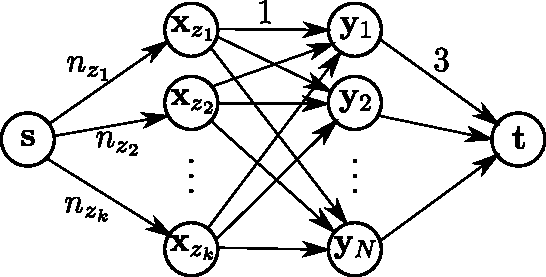
\includegraphics[width=0.6\linewidth]{figures/flow}
	\caption{Flow problem to compute and optimal assignment.}
\end{figure}

We first show the equivalence between this problem and and the construction of an assignment. Given some optimal assignment $(n_v)$, define the flow $f:E\to \mathbb{N}$ that saturates every edge from $\mathbf{s}$ or to $\mathbf{t}$, takes value $1$ on the edge between $\mathbf{x}_z$ and $\mathbf{y}_i$ if partition $i$ is stored in some node of the zone $z$, and $0$ otherwise. One can easily check that $f$ thus defined is indeed a flow and is maximum.

Reciprocally, by the existence of maximum flows constructed from optimal assignments, any maximum flow must saturate the edges linked to the source or the sink. It can only take value 0 or 1 on the other edge, and every partition vertex is associated to exactly three distinct zone vertices. Every zone is associated to exactly $n_z$ partitions.

A maximum flow can be constructed using, for instance, Dinic's algorithm. This algorithm works by discovering augmenting path to iteratively increase the flow. During the exploration of the graph to find augmenting path, we can shuffle the order of enumeration of the neighbours to spread the associations between zones and partitions.

Once we have such association, we can randomly distribute the $n_z$ edges picked for every zone $z$ to its nodes $v\in z$ such that every such $v$ gets $n_z$ edges. This defines an optimal assignment of partitions to nodes.


\subsection{Minimal transfer}

Assume that there was a previous assignment $(T'_i)_{1\le i\le N}$ corresponding to utilizations $(n'_v)_{v\in V}$. We would like the new computed assignment $(T_i)_{1\le i\le N}$ from some $(n_v)_{v\in V}$ to minimize the number of partitions that need to be transferred. We can imagine two different objectives corresponding to different hypotheses: 
\begin{equation}
	\tag{H3A}
	\label{hyp:A}
	\text{\emph{Transfers between different zones cost much more than inside a zone.}}
\end{equation}
\begin{equation}
	\tag{H3B}
	\label{hyp:B}
	\text{\emph{Changing zone is not the largest cost when transferring a partition.}}
\end{equation}

In case $A$, our goal will be to minimize the number of changes of zone in the assignment of partitions to zone. More formally, we will maximize the quantity
$$
Q_Z := 
\sum_{1\le i\le N} 
\#\{z\in Z ~|~ z\cap T_i \neq \emptyset, z\cap T'_i \neq \emptyset \}
.$$

In case $B$, our goal will be to minimize the number of changes of nodes in the assignment of partitions to nodes. We will maximize the quantity
$$
Q_V :=
\sum_{1\le i\le N} \#(T_i \cap T'_i).
$$

It is tempting to hope that there is a way to maximize both quantity, that having the least discrepancy in terms of nodes will lead to the least discrepancy in terms of zones. But this is actually wrong! We propose the following counter-example to convince the reader:

We consider eight nodes $a, a', b, c, d, d', e, e'$ belonging to five different zones $\{a,a'\}, \{b\}, \{c\}, \{d,d'\}, \{e, e'\}$. We take three partitions ($N=3$), that are originally assigned with some utilization $(n'_v)_{v\in V}$ as follows:
$$
T'_1=(a,b,c) \qquad
T'_2=(a',b,d) \qquad 
T'_3=(b,c,e).
$$
This assignment, with updated utilizations $(n_v)_{v\in V}$ minimizes the number of zone changes:
$$
T_1=(d,b,c) \qquad
T_2=(a,b,d) \qquad 
T_3=(b,c,e').
$$
This one, with the same utilization, minimizes the number of node changes:
$$
T_1=(a,b,c) \qquad
T_2=(e',b,d) \qquad 
T_3=(b,c,d').
$$
One can check that in this case, it is impossible to minimize both the number of zone and node changes.

Because of the redundancy constraint, we cannot use a greedy algorithm to just replace nodes in the triplets to try to get the new utilization rate: this could lead to blocking situation where there is still a hole to fill in a triplet but no available node satisfies the zone separation constraint. To circumvent this issue, we propose an algorithm based on finding cycles in a graph encoding of the assignment. As in section \ref{sec:opt_assign}, we can explore the neigbours in a random order in the graph algorithms, to spread the triplets distribution.


\subsubsection{Minimizing the zone discrepancy}


First, notice that, given an assignment of partitions to \emph{zones}, it is easy to deduce an assignment to \emph{nodes} that minimizes the number of transfers for this zone assignment: For every zone $z$ and every node $v\in z$, pick in any way a set $P_v$ of partitions that where assigned to $v$ in $T'$, to $z_v$ in $T$, with the cardinality of $P_v$ smaller than $n_v$. Once all these sets are chosen, complement the assignment to reach the right utilization for every node. If $\#P_v > n_v$, it means that all the partitions that could stay in $v$ (i.e. that were already in $v$ and are still assigned to its zone) do stay in $v$. If $\#P_v = n_v$, then $n_v$ partitions stay in $v$, which is the number of partitions that need to be in $v$ in the end. In both cases, we could not hope for better given the partition to zone assignment.

Our goal now is to find a assignment of partitions to zones that minimizes the number of zone transfers. To do so we are going to represent an assignment as a graph.

Let $G_T=(X,E_T)$ be the directed weighted graph with vertices $(\mathbf{x}_i)_{1\le i\le N}$ and $(\mathbf{y}_z)_{z\in Z}$. For any $1\le i\le N$ and $z\in Z$, $E_T$ contains  the arc:
\begin{itemize}
	\item $(\mathbf{x}_i, \mathbf{y}_z, +1)$, if $z$ appears in $T_i'$ and $T_i$;
	\item $(\mathbf{x}_i, \mathbf{y}_z, -1)$, if $z$ appears in $T_i$ but not in $T'_i$;
	\item $(\mathbf{y}_z, \mathbf{x}_i, -1)$, if $z$ appears in $T'_i$ but not in $T_i$;
	\item $(\mathbf{y}_z, \mathbf{x}_i, +1)$, if $z$ does not appear in $T'_i$ nor in $T_i$.
\end{itemize}
In other words, the orientation of the arc encodes whether partition $i$ is stored in zone $z$ in the assignment $T$ and the weight $\pm 1$ encodes whether this corresponds to what happens in the assignment $T'$.

\begin{figure}[t]
	\centering
	\begin{minipage}{.40\linewidth}
		\centering
		\includegraphics[width=.8\linewidth]{figures/mini_zone}
	\end{minipage}
	\begin{minipage}{.55\linewidth}
		\centering
		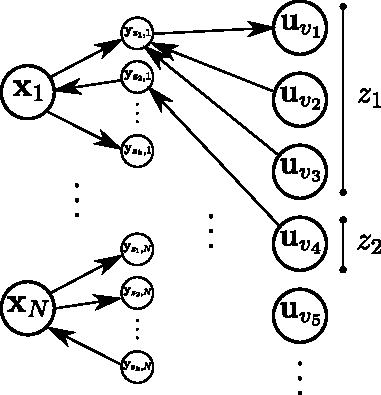
\includegraphics[width=.8\linewidth]{figures/mini_node}
	\end{minipage}
	\caption{On the left: the graph $G_T$ encoding an assignment to minimize the zone discrepancy. On the right: the graph $G_T$ encoding an assignment to minimize the node discrepancy.}
\end{figure}


Notice that at every partition, there are three outgoing arcs, and at every zone, there are $n_z$ incoming arcs. Moreover, if $w(e)$ is the weight of an arc $e$, define the weight of $G_T$ by
\begin{align*}
w(G_T) := \sum_{e\in E} w(e) &= \#Z \times N - 4 \sum_{1\le i\le N} \#\{z\in Z ~|~ z\cap T_i = \emptyset, z\cap T'_i \neq \emptyset\}	\\
&=\#Z \times N - 4 \sum_{1\le i\le N} 3- \#\{z\in Z ~|~ z\cap T_i \neq \emptyset, z\cap T'_i \neq \emptyset\} \\
&= (\#Z-12)N + 4 Q_Z.
\end{align*}
Hence maximizing $Q_Z$ is equivalent to maximizing $w(G_T)$.

Assume that their exist some assignment $T^*$ with the same utilization $(n_v)_{v\in V}$. Define $G_{T^*}$ similarly and consider the set $E_\mathrm{Diff} = E_T \setminus E_{T^*}$ of arcs that appear only in $G_T$. Since all vertices have the same number of incoming arcs in $G_T$ and $G_{T^*}$, the vertices of the graph $(X, E_\mathrm{Diff})$ must all have the same number number of incoming and outgoing arrows. So $E_\mathrm{Diff}$ can be expressed as a union of disjoint cycles. Moreover, the edges of $E_\mathrm{Diff}$ must appear in $E_{T^*}$ with reversed orientation and opposite weight. Hence, we have
$$
 w(G_T) - w(G_{T^*}) = 2 \sum_{e\in E_\mathrm{Diff}} w(e). 
$$
Hence, if $T$ is not optimal, there exists some $T^*$ with $w(G_T) < w(G_{T^*})$, and by the considerations above, there must exist a cycle in $E_\mathrm{Diff}$, and hence in $G_T$, with negative weight. If we reverse the edges and weights along this cycle, we obtain some graph. Since we did not change the incoming degree of any vertex, this is the graph encoding of some valid assignment $T^+$ such that $w(G_{T^+}) > w(G_T)$. We can iterate this operation until there is no other assignment $T^*$ with larger weight, that is until we obtain an optimal assignment.



\subsubsection{Minimizing the node discrepancy}

We will follow an approach similar to the one where we minimize the zone discrepancy. Here we will directly obtain a node assignment from a graph encoding.

Let $G_T=(X,E_T)$ be the directed weighted graph with vertices $(\mathbf{x}_i)_{1\le i\le N}$, $(\mathbf{y}_{z,i})_{z\in Z, 1\le i\le N}$ and $(\mathbf{u}_v)_{v\in V}$. For any $1\le i\le N$ and $z\in Z$, $E_T$ contains  the arc:
\begin{itemize}
	\item $(\mathbf{x}_i, \mathbf{y}_{z,i}, 0)$, if $z$ appears in $T_i$;
	\item $(\mathbf{y}_{z,i}, \mathbf{x}_i, 0)$, if $z$ does not appear in $T_i$.
\end{itemize}
For any $1\le i\le N$ and $v\in V$, $E_T$ contains  the arc:
\begin{itemize}
	\item $(\mathbf{y}_{z_v,i}, \mathbf{u}_v, +1)$, if $v$ appears in $T_i'$ and $T_i$;
	\item $(\mathbf{y}_{z_v,i}, \mathbf{u}_v, -1)$, if $v$ appears in $T_i$ but not in $T'_i$;
	\item $(\mathbf{u}_v, \mathbf{y}_{z_v,i}, -1)$, if $v$ appears in $T'_i$ but not in $T_i$;
	\item $(\mathbf{u}_v, \mathbf{y}_{z_v,i}, +1)$, if $v$ does not appear in $T'_i$ nor in $T_i$.
\end{itemize}
Every vertex $\mathbb{x}_i$ has outgoing degree 3, every vertex $\mathbf{y}_{z,v}$ has outgoing degree 1, and every vertex $\mathbf{u}_v$ has incoming degree $n_v$. 
Remark that any graph respecting these degree constraints is the encoding of a valid assignment with utilizations $(n_v)_{v\in V}$, in particular no partition is stored in two nodes of the same zone.

We define $w(G_T)$ similarly:
\begin{align*}
	w(G_T) := \sum_{e\in E_T} w(e) &= \#V \times N - 4\sum_{1\le i\le N} 3-\#(T_i\cap T'_i) \\
	&= (\#V-12)N + 4Q_V.
\end{align*}

Exactly like in the previous section, the existence of an assignment with larger weight implies the existence of a negatively weighted cycle in $G_T$. Reversing this cycle gives us the encoding of a valid assignment with a larger weight. Iterating this operation yields an optimal assignment.


\subsubsection{Linear combination of both criteria}

In the graph $G_T$ defined in the previous section, instead of having weights $0$ and $\pm 1$, we could be having weights $\pm\alpha$ between $\mathbf{x}$ and  $\mathbf{y}$ vertices, and weights $\pm\beta$ between $\mathbf{y}$ and  $\mathbf{u}$ vertices, for some $\alpha,\beta>0$ (we have positive weight if the assignment corresponds to $T'$ and negative otherwise). Then
\begin{align*}
	w(G_T) &= \sum_{e\in E_T} w(e) = 
	\alpha \big( (\#Z-12)N + 4 Q_Z\big) + 
	\beta \big( (\#V-12)N + 4 Q_V\big) \\
	&= \mathrm{const}+ 4(\alpha Q_Z + \beta Q_V).
\end{align*}
So maximizing the weight of such graph encoding would be equivalent to maximizing a linear combination of $Q_Z$ and $Q_V$.


\subsection{Algorithm}
We give a high level description of the algorithm to compute an optimal 3-strict assignment. The operations appearing at lines 1,2,4 are respectively described by Algorithms \ref{alg:util},\ref{alg:opt} and \ref{alg:mini}.



\begin{algorithm}[H]
	\caption{Optimal 3-strict assignment}
	\label{alg:total}
	\begin{algorithmic}[1]
	\Function{Optimal 3-strict assignment}{$N$, $(c_v)_{v\in V}$, $T'$}
		\State $(n_v)_{v\in V} \leftarrow$ \Call{Compute optimal utilization}{$N$, $(c_v)_{v\in V}$}
		\State $(T_i)_{1\le i\le N} \leftarrow$ \Call{Compute candidate assignment}{$N$, $(n_v)_{v\in V}$}
		\If {there was a previous assignment $T'$}
			\State $T \leftarrow$ \Call{Minimization of transfers}{$(T_i)_{1\le i\le N}$, $(T'_i)_{1\le i\le N}$}
		\EndIf
		\State \Return $T$.
	\EndFunction
	\end{algorithmic}
\end{algorithm}

We give some considerations of worst case complexity for these algorithms. In the following, we assume $N>\#V>\#Z$. The complexity of Algorithm \ref{alg:total} is $O(N^3\# Z)$ if we assume \eqref{hyp:A} and $O(N^3 \#Z \#V)$ if we assume \eqref{hyp:B}.

Algorithm \ref{alg:util} can be implemented with complexity $O(\#V^2)$. The complexity of the function call at line \ref{lin:subutil} is $O(\#V)$. The difference between the sum of the subutilizations and $3N$ is at most the sum of the rounding errors when computing the $\hat{n}_v$. Hence it is bounded by $\#V$ and the loop at line \ref{lin:loopsub} is iterated at most $\#V$ times. Finding the minimizing $v$ at line \ref{lin:findmin} takes $O(\#V)$ operations (naively, we could also use a heap).

Algorithm \ref{alg:opt} can be implemented with complexity $O(N^3\times \#Z)$. The flow graph has $O(N+\#Z)$ vertices and $O(N\times \#Z)$ edges. Dinic's algorithm has complexity $O(\#\mathrm{Vertices}^2\#\mathrm{Edges})$ hence in our case it is $O(N^3\times \#Z)$.
 
Algorithm \ref{alg:mini} can be implented with complexity $O(N^3\# Z)$ under \eqref{hyp:A} and $O(N^3 \#Z \#V)$ under \eqref{hyp:B}.
The graph $G_T$ has $O(N)$ vertices and $O(N\times \#Z)$ edges under assumption \eqref{hyp:A} and respectively $O(N\times \#Z)$ vertices and $O(N\times \#V)$ edges under assumption \eqref{hyp:B}. The loop at line \ref{lin:repeat} is iterated at most $N$ times since the distance between $T$ and $T'$ decreases at every iteration. Bellman-Ford algorithm has complexity $O(\#\mathrm{Vertices}\#\mathrm{Edges})$, which in our case amounts to $O(N^2\# Z)$ under \eqref{hyp:A} and $O(N^2 \#Z \#V)$ under \eqref{hyp:B}.
 
\begin{algorithm}
	\caption{Computation of the optimal utilization}
	\label{alg:util}
	\begin{algorithmic}[1]
\Function{Compute optimal utilization}{$N$, $(c_v)_{v\in V}$}
	\State $(\hat{n}_v)_{v\in V} \leftarrow $ \Call{Compute subutilization}{$N$, $(c_v)_{v\in V}$} \label{lin:subutil}
	\While{$\sum_{v\in V} \hat{n}_v < 3N$} \label{lin:loopsub}
	\State Pick $v\in V$ minimizing $\frac{c_v}{\hat{n}_v+1}$ and such that
		$\sum_{v'\in z_v} \hat{n}_{v'} < N$ \label{lin:findmin}
		\State $\hat{n}_v \leftarrow \hat{n}_v+1$
	\EndWhile
	\State \Return $(\hat{n}_v)_{v\in V}$
\EndFunction
\State

\Function{Compute subutilization}{$N$, $(c_v)_{v\in V}$}
		\State $R \leftarrow 3$
\For{$v\in V$}
\State $\hat{n}_v \leftarrow \mathrm{unset}$
\EndFor
\For{$z\in Z$}
\State $c_z \leftarrow \sum_{v\in z} c_v$
\EndFor
\State $C \leftarrow \sum_{z\in Z} c_z$
\While{$\exists z \in Z$ such that $R\times c_{z} > C$}
\For{$v\in z$}
\State $\hat{n}_v \leftarrow \left\lfloor \frac{c_v}{c_z} N \right\rfloor$
\EndFor
\State $C \leftarrow C-c_z$
\State $R\leftarrow R-1$
\EndWhile
\For{$v\in V$}
\If{$\hat{n}_v = \mathrm{unset}$}
\State $\hat{n}_v \leftarrow \left\lfloor \frac{Rc_v}{C} N \right\rfloor$
\EndIf
\EndFor
\State \Return $(\hat{n}_v)_{v\in V}$
\EndFunction
	\end{algorithmic}
\end{algorithm}

\begin{algorithm}
	\caption{Computation of a candidate assignment}
	\label{alg:opt}
	\begin{algorithmic}[1]
		\Function{Compute candidate assignment}{$N$, $(n_v)_{v\in V}$}
		\State Compute the flow graph $G$
		\State Compute the maximal flow $f$ using Dinic's algorithm with randomized neighbours enumeration
		\State Construct the assignment $(T_i)_{1\le i\le N}$ from $f$
		\State \Return $(T_i)_{1\le i\le N}$
		\EndFunction
	\end{algorithmic}
\end{algorithm}


\begin{algorithm}
	\caption{Minimization of the number of transfers}
	\label{alg:mini}
	\begin{algorithmic}[1]
		\Function{Minimization of transfers}{$(T_i)_{1\le i\le N}$, $(T'_i)_{1\le i\le N}$}
		\State Construct the graph encoding $G_T$
		\Repeat \label{lin:repeat}
		\State Find a negative cycle $\gamma$ using Bellman-Ford algorithm on $G_T$
		\State Reverse the orientations and weights of edges in $\gamma$
		\Until{no negative cycle is found}
		\State Update $(T_i)_{1\le i\le N}$ from $G_T$
		\State \Return $(T_i)_{1\le i\le N}$
		\EndFunction
	\end{algorithmic}
\end{algorithm}

\newpage

\section{Computation of a 3-non-strict assignment}

\subsection{Choices of optimality}

In this mode, we primarily want to store every partition on three nodes, and only secondarily try to spread the nodes among different zone. So we make the choice of not taking the zone repartition in the criterion of optimality.

We try to maximize $s^*$ defined in \eqref{eq:optimal}. So we can compute the optimal utilizations $(n_v)_{v\in V}$ with the only constraint that $n_v \le N$ for every node $v$. As in the previous section, we start with a sub-utilization proportional to $c_v$ (and capped at $N$), and we iteratively increase the $\hat{n}_v$ that is less than $N$ and maximizes the quantity $c_v/(\hat{n}_v+1)$, until the total sum is $3N$.

\subsection{Computation of a candidate assignment}

To compute a candidate assignment (that does not optimize zone spreading nor distance to a previous assignment yet), we can use the folowing flow problem.

Define the oriented weighted graph $(X,E)$. The set of vertices $X$ contains the source $\mathbf{s}$, the sink $\mathbf{t}$, vertices 
$\mathbf{x}_p, \mathbf{u}^+_p, \mathbf{u}^-_p$ for every partition $p$, vertices $\mathbf{y}_{p,z}$ for every partition $p$ and zone $z$, and vertices $\mathbf{z}_v$ for every node $v$. 

The set of edges is composed of the following arcs:
\begin{itemize}
	\item ($\mathbf{s}$,$\mathbf{x}_p$, 3) for every partition $p$;
	\item ($\mathbf{x}_p$,$\mathbf{u}^+_p$, 3) for every partition $p$;
	\item ($\mathbf{x}_p$,$\mathbf{u}^-_p$, 2) for every partition $p$;
	\item ($\mathbf{u}^+_p$,$\mathbf{y}_{p,z}$, 1) for every partition $p$ and zone $z$;
	\item ($\mathbf{u}^-_p$,$\mathbf{y}_{p,z}$, 2) for every partition $p$ and zone $z$;
	\item ($\mathbf{y}_{p,z}$,$\mathbf{z}_v$, 1) for every partition $p$, zone $z$ and node $v\in z$;
	\item ($\mathbf{z}_v$, $\mathbf{t}$, $n_v$) for every node $v$;
\end{itemize}

One can check that any maximal flow in this graph corresponds to an assignment of partitions to nodes. In such a flow, all the arcs from $\mathbf{s}$ and to $\mathbf{t}$ are saturated. The arc from $\mathbf{y}_{p,z}$ to $\mathbf{z}_v$ is saturated if and only if $p$ is associated to~$v$. 
Finally the flow from $\mathbf{x}_p$ to $\mathbf{y}_{p,z}$ can go either through $\mathbf{u}^+_p$ or $\mathbf{u}^-_p$.



\subsection{Maximal spread and minimal transfers}
Notice that if the arc $\mathbf{u}_p^+\mathbf{y}_{p,z}$ is not saturated but there is some flow in $\mathbf{u}_p^-\mathbf{y}_{p,z}$, then it is possible to transfer a unit of flow from the path  $\mathbf{x}_p\mathbf{u}_p^-\mathbf{y}_{p,z}$ to the path $\mathbf{x}_p\mathbf{u}_p^+\mathbf{y}_{p,z}$. So we can always find an equivalent maximal flow $f^*$ that uses the path through $\mathbf{u}_p^-$ only if the path through $\mathbf{u}_p^+$ is saturated.

We will use this fact to consider the amount of flow going through the vertices $\mathbf{u}^+$ as a measure of how well the partitions are spread over nodes belonging to different zones. If the partition $p$ is associated to 3 different zones, then a flow of 3 will cross $\mathbf{u}_p^+$ in $f^*$ (i.e. a flow of 0 will cross $\mathbf{u}_p^+$). If $p$ is associated to two zones, a flow of $2$ will cross $\mathbf{u}_p^+$. If $p$ is associated to a single zone, a flow of $1$ will cross $\mathbf{u}_p^+$.

Let $N_1, N_2, N_3$ be the number of partitions associated to respectively 1,2 and 3 distinct zones. We will optimize a linear combination of these variables using the discovery of positively weighted circuits in a graph.

At the same step, we will also optimize the distance to a previous assignment $T'$. Let $\alpha> \beta> \gamma \ge 0$ be three parameters.

Given the flow $f$, let $G_f=(X',E_f)$ be the multi-graph where $X' = X\setminus\{\mathbf{s},\mathbf{t}\}$. The set $E_f$ is composed of the arcs:
\begin{itemize}
\item As many arcs from $(\mathbf{x}_p, \mathbf{u}^+_p,\alpha), (\mathbf{x}_p, \mathbf{u}^+_p,\beta), (\mathbf{x}_p, \mathbf{u}^+_p,\gamma)$ (selected in this order) as there is flow crossing $\mathbf{u}^+_p$ in $f$;
\item As many arcs from $(\mathbf{u}^+_p, \mathbf{x}_p,-\gamma), (\mathbf{u}^+_p, \mathbf{x}_p,-\beta), (\mathbf{u}^+_p, \mathbf{x}_p,-\alpha)$ (selected in this order) as there is flow crossing $\mathbf{u}^-_p$ in $f$;
\item  As many copies of $(\mathbf{x}_p, \mathbf{u}^-_p,0)$ as there is flow through $\mathbf{u}^-_p$;
\item  As many copies of $(\mathbf{u}^-_p,\mathbf{x}_p,0)$ so that the number of arcs between these two vertices is 2;
\item $(\mathbf{u}^+_p,\mathbf{y}_{p,z}, 0)$ if the flow between these vertices is 1, and the opposite arc otherwise;
\item as many copies of $(\mathbf{u}^-_p,\mathbf{y}_{p,z}, 0)$ as the flow between these vertices, and as many copies of the opposite arc as 2~$-$~the flow;
\item $(\mathbf{y}_{p,z},\mathbf{z}_v, \pm1)$ if it is saturated in $f$, with $+1$ if $v\in T'_p$ and $-1$ otherwise;
\item $(\mathbf{z}_v,\mathbf{y}_{p,z}, \pm1)$ if it is not saturated in $f$, with $+1$ if $v\notin T'_p$ and $-1$ otherwise.
\end{itemize}
To summarize, arcs are oriented left to right if they correspond to a presence of flow in $f$, and right to left if they correspond to an absence of flow. They are positively weighted if we want them to stay at their current state, and negatively if we want them to switch. Let us compute the weight of such graph.

\begin{multline*}
	w(G_f)  = \sum_{e\in E_f} w(e_f)  \\
	= 
	(\alpha - \beta -\gamma) N_1 + (\alpha +\beta - \gamma) N_2 + (\alpha+\beta+\gamma) N_3 
	\\ + 
	\#V\times N - 4 \sum_p 3-\#(T_p\cap T'_p) \\ 
	=(\#V-12+\alpha-\beta-\gamma)\times N + 4Q_V + 2\beta N_2 + 2(\beta+\gamma) N_3 \\
\end{multline*}

As for the mode 3-strict, one can check that the difference of two such graphs corresponding to the same $(n_v)$ is always eulerian. Hence we can navigate in this class with the same greedy algorithm that discovers positive cycles and flips them.

The function that we optimize is 
$$
2Q_V +  \beta N_2 + (\beta+\gamma) N_3.
$$
The choice of parameters $\beta$ and $\gamma$ should be lead by the following question: For $\beta$, where to put the tradeoff between zone dispersion and distance to the previous configuration? For $\gamma$, do we prefer to have more partitions spread between 2 zones, or have less between at least 2 zones but more between 3 zones.

The quantity $Q_V$ varies between $0$ and $3N$, it should be of order $N$. The quantity $N_2+N_3$ should also be of order $N$ (it is exactly $N$ in the strict mode). So the two terms of the function are comparable. 


\bibliography{optimal_layout} 
\bibliographystyle{ieeetr}

\end{document}



